\chapter[Orçamento do Projeto]{Orçamento do Projeto}

\section{Mês de abril}
\begin{figure}[H]
	\centering
	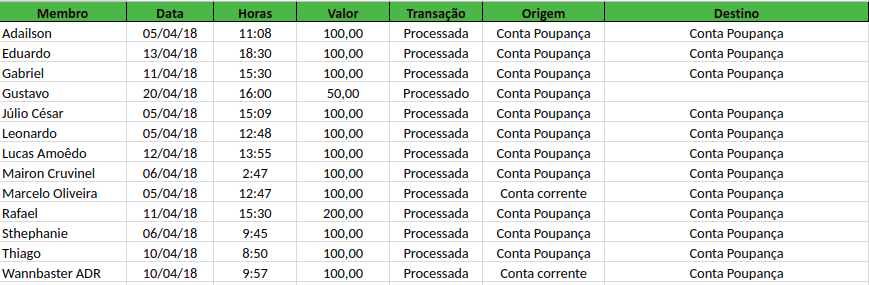
\includegraphics[width=17cm]{figuras/entrada_ativos.png}
	\caption{Entrada de ativos financeiros} \label{entrada_ativos}
\end{figure}

\begin{figure}[H]
	\centering
	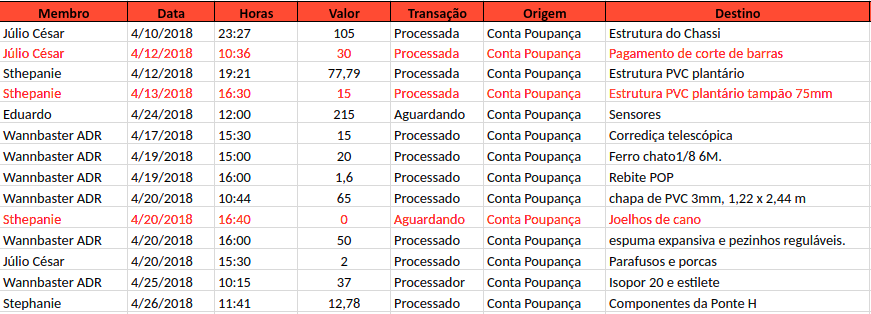
\includegraphics[width=17cm]{figuras/saida_ativos.png}
	\caption{Saída de ativos financeiros} \label{saida_ativos}
\end{figure}

\begin{figure}[H]
	\centering
	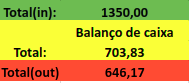
\includegraphics[width=7cm]{figuras/balanco_abril.png}
	\caption{Balanço de Caixa} \label{balanco_abril}
\end{figure}

\section{Mês de maio}

\begin{figure}[H]
	\centering
	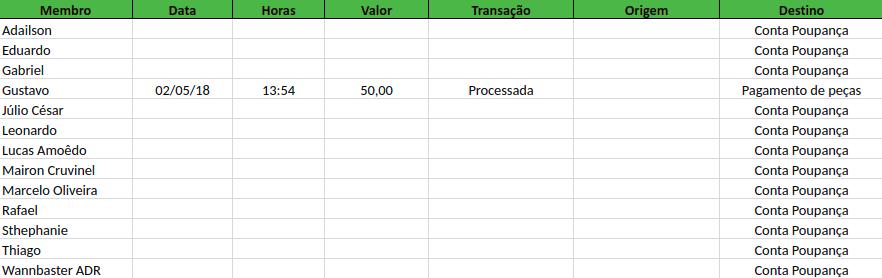
\includegraphics[width=17cm]{figuras/entrada_ativos_maio.png}
	\caption{Entrada de ativos financeiros} \label{entrada_ativos_maio}
\end{figure}

\begin{figure}[H]
	\centering
	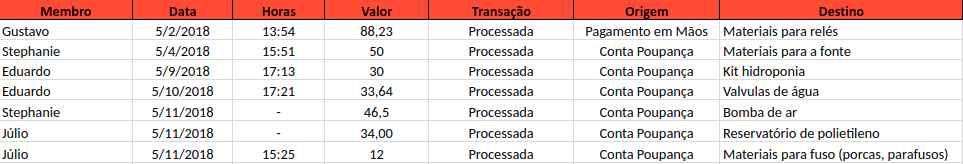
\includegraphics[width=17cm]{figuras/saida_ativos_maio.png}
	\caption{Saída de ativos financeiros} \label{saida_ativos_maio}
\end{figure}

\begin{figure}[H]
	\centering
	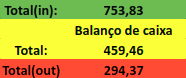
\includegraphics[width=7cm]{figuras/balanco_maio.png}
	\caption{Balanço de Caixa} \label{balanco_maio}
\end{figure}

\section{Mês de junho}

\begin{figure}[H]
	\centering
	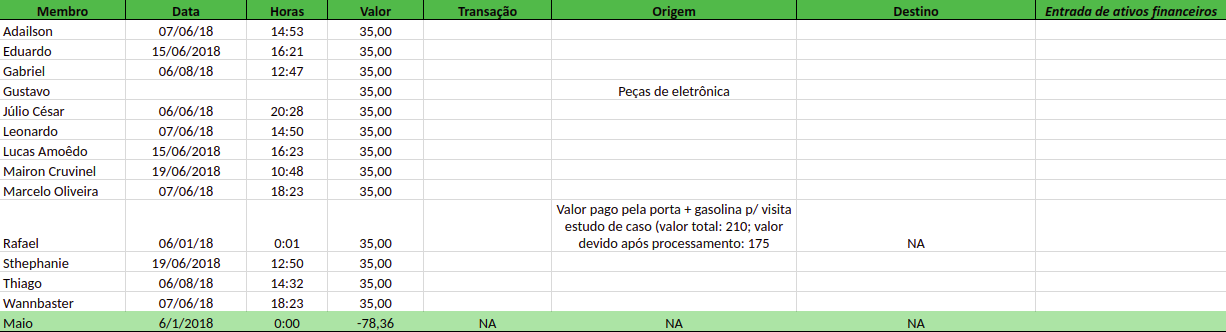
\includegraphics[width=17cm]{figuras/entrada_ativos_junho.png}
	\caption{Entrada de ativos financeiros} \label{entrada_ativos_junho}
\end{figure}

\begin{figure}[H]
	\centering
	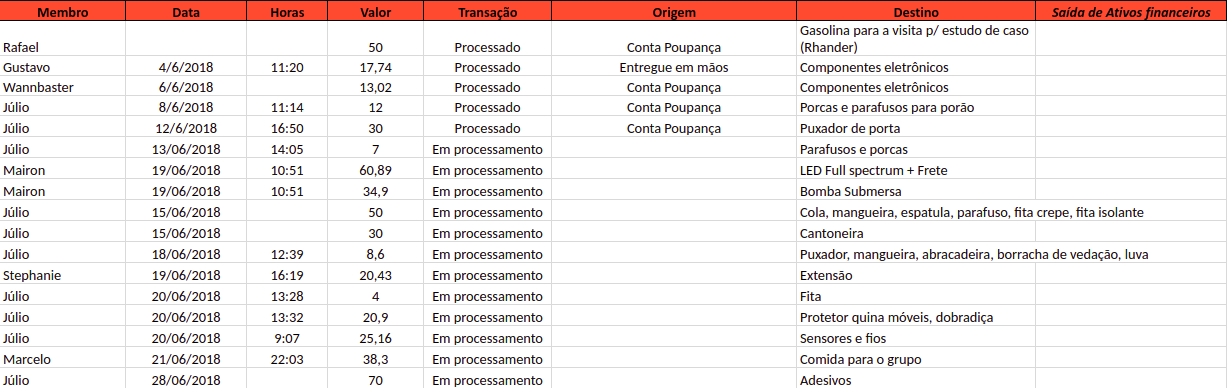
\includegraphics[width=17cm]{figuras/saida_ativos_junho.png}
	\caption{Saída de ativos financeiros} \label{saida_ativos_junho}
\end{figure}

\begin{figure}[H]
	\centering
	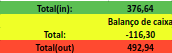
\includegraphics[width=7cm]{figuras/balanco_junho.png}
	\caption{Balanço de Caixa} \label{balanco_junho}
\end{figure}